
% Autoría principal: Mario Zambrano.

\subsection{Estadísticas descriptivas por mecanismo y tamaño}

Se analizaron 2000 mediciones de latencia RTT, distribuidas
entre TCP y gRPC con mensajes de 100 y 10240 bytes.
Para cada combinación se realizaron cinco corridas
de 100 envíos, obteniendo 500 mediciones por caso.

A partir de los archivos CSV se calcularon la media,
mediana, desviación estándar y percentil 95 (P95).
Estos cálculos se realizaron mediante el script
\texttt{analisis\_resultados.py}, utilizando pandas.
Los resultados se muestran en la
Tabla~\ref{tab:estadisticas_rtt}.

\begin{table}[htbp]
\centering
\small
\resizebox{\linewidth}{!}{%
\begin{tabular}{llrrrrr}
\toprule
Mecanismo & Carga útil & $n$ & Media (ms) & Mediana (ms) & DE (ms) & P95 (ms) \\
\midrule
TCP & 100 B & 500 & 0.122 & 0.113 & 0.028 & 0.185 \\
TCP & 10 KiB (10240 B) & 500 & 0.197 & 0.186 & 0.039 & 0.282 \\
gRPC & 100 B & 500 & 0.547 & 0.489 & 0.231 & 0.819 \\
gRPC & 10 KiB (10240 B) & 500 & 0.564 & 0.533 & 0.110 & 0.758 \\
\bottomrule
\end{tabular}%
}
\caption{Latencia RTT por mecanismo y tamaño de carga útil. DE: desviación estándar muestral; P95: percentil 95.}
\label{tab:estadisticas_rtt}
\end{table}


En las pruebas realizadas, TCP presentó una latencia
media menor que gRPC con los dos tamaños de mensaje.
Lo mismo ocurrió con las medianas y los valores del
percentil 95.

Al aumentar el tamaño del mensaje de 100 a 10240 bytes,
la latencia media también aumentó en ambos casos.
Este cambio fue mayor en TCP, mientras que en gRPC
la diferencia entre los dos tamaños fue más pequeña.

También se encontraron diferencias en la dispersión
de los tiempos. gRPC registró una desviación estándar
mayor que TCP, especialmente con mensajes de 100 bytes.
Esto indica que sus tiempos de respuesta fueron menos
uniformes durante las pruebas.

Las posibles razones de estas diferencias se
analizarán en la sección de discusión.

\subsection{Rendimiento: mensajes por segundo}

Además de medir la latencia, se calculó cuántos mensajes
podía procesar cada implementación por segundo.
Para ello, se dividió la cantidad de mensajes
confirmados entre el tiempo total de cada corrida.

En la Tabla~\ref{tab:rendimiento} se presentan
los promedios de rendimiento y sus desviaciones
estándar, calculados a partir de las cinco
corridas realizadas para cada caso.

\begin{table}[htbp]
\centering
\small
\resizebox{\linewidth}{!}{%
\begin{tabular}{llrrr}
\toprule
Mecanismo & Carga útil & Corridas & Media (mensajes/s) & DE (mensajes/s) \\
\midrule
TCP & 100 B & 5 & 576.43 & 4.03 \\
TCP & 10 KiB (10240 B) & 5 & 533.24 & 17.70 \\
gRPC & 100 B & 5 & 442.64 & 21.42 \\
gRPC & 10 KiB (10240 B) & 5 & 431.98 & 19.71 \\
\bottomrule
\end{tabular}%
}
\caption{Rendimiento observado, calculado como mensajes confirmados divididos entre la duración de cada corrida; media y desviación estándar de cinco corridas.}
\label{tab:rendimiento}
\end{table}


TCP obtuvo un rendimiento medio superior al de gRPC
con ambos tamaños de mensaje. También se observó
que el número de mensajes procesados por segundo
disminuyó al utilizar la carga de 10240 bytes.

En cuanto a la variación entre corridas, TCP con
mensajes de 100 bytes presentó los resultados más
uniformes. Por su parte, gRPC registró diferencias
mayores entre las repeticiones.

Es importante aclarar que el rendimiento y el RTT
no se calculan de la misma manera. El rendimiento
considera el tiempo completo de cada corrida,
incluyendo las operaciones de registro realizadas
por el cliente. Por eso, no se obtiene simplemente
dividiendo uno entre la latencia media.

\subsection{Gráfico de cajas de latencias}

Para observar mejor la distribución de los tiempos,
se generó el diagrama de cajas de la
Figura~\ref{fig:boxplot}. Este gráfico permite
comparar las medianas, la dispersión y los
valores atípicos de las mediciones.

\begin{figure}[H]
    \centering
    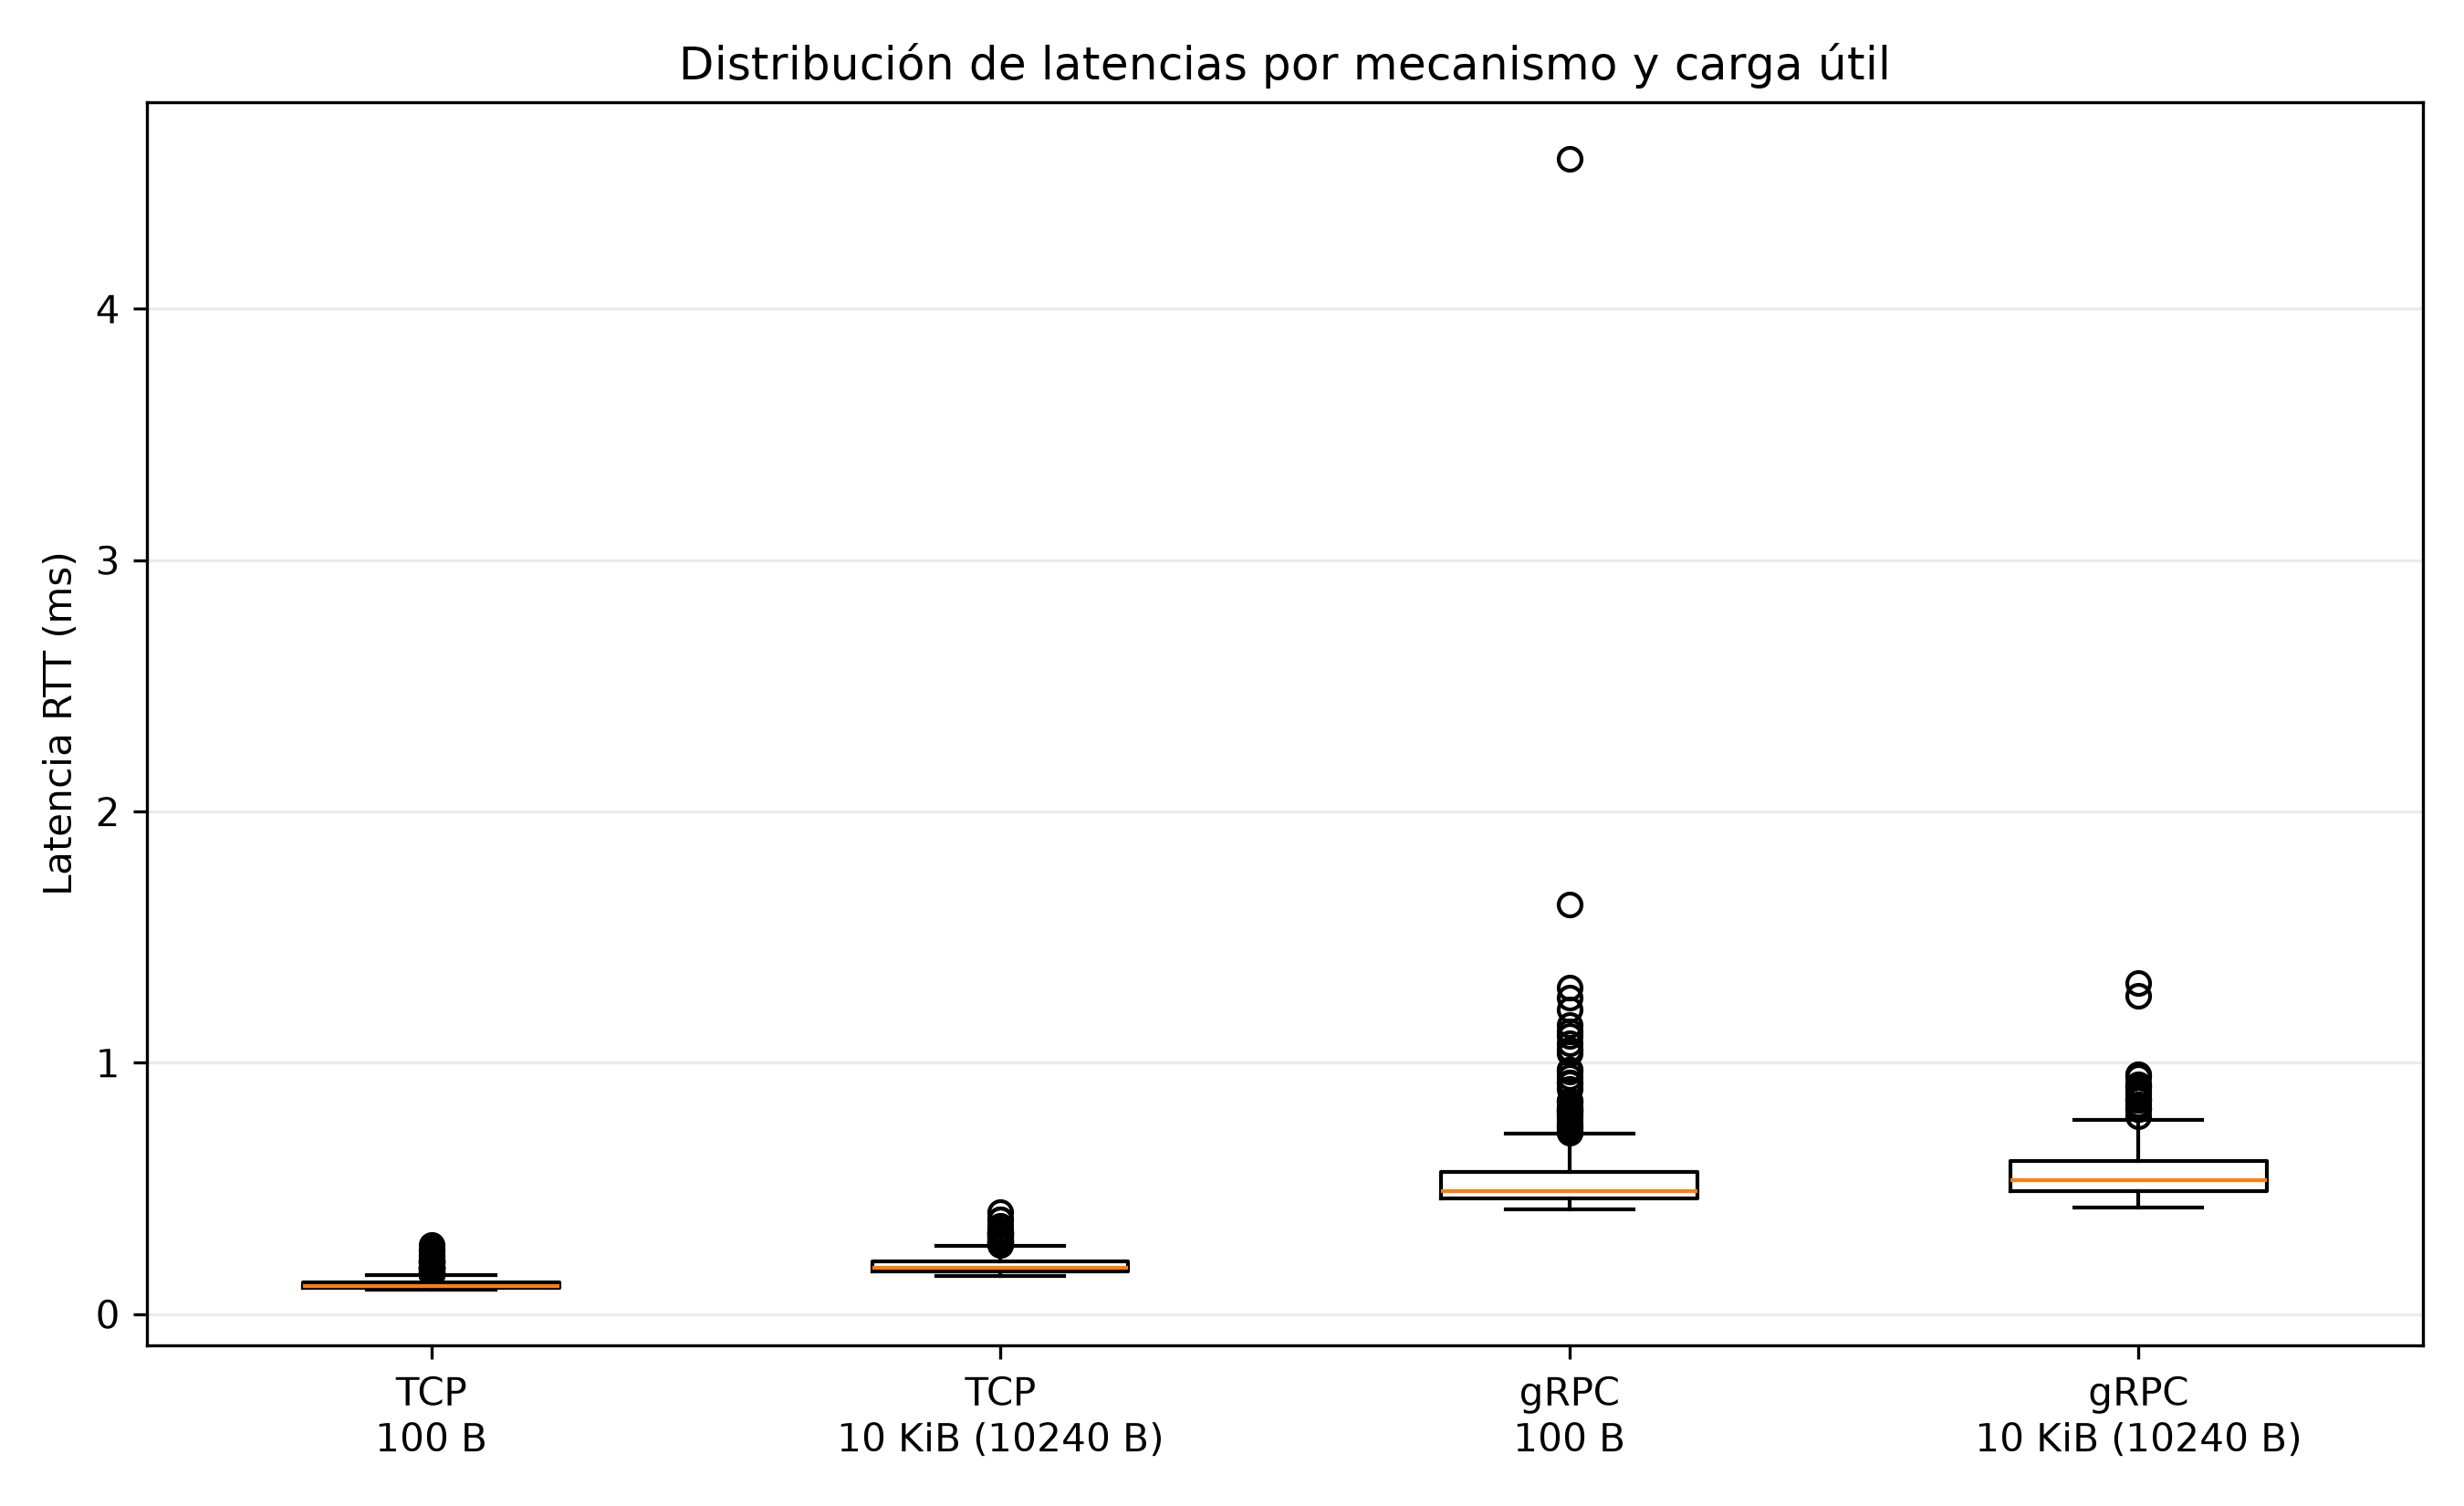
\includegraphics[width=0.95\linewidth]
    {figures/boxplot.png}
    \caption{Distribución de las latencias RTT de
    TCP y gRPC con mensajes de 100 bytes y 10 KiB.
    Gráfico generado a partir de los CSV originales.}
    \label{fig:boxplot}
\end{figure}

Como se observa en el gráfico, los tiempos de TCP
se concentran en valores más bajos que los de gRPC.
También se aprecia que las mediciones de gRPC
presentan una mayor dispersión, principalmente
con mensajes de 100 bytes.

En esta última condición aparecen algunos valores
atípicos que se alejan del resto de las mediciones.
Se decidió conservarlos porque forman parte de
los datos obtenidos durante la ejecución.
Por tanto, también se consideraron en los
cálculos estadísticos.

El gráfico permite identificar estas diferencias,
pero no es suficiente para determinar qué provocó
cada aumento de latencia.

\subsection{Gráfico de barras con intervalos}

La Figura~\ref{fig:barras} muestra una comparación
de la latencia media para los dos mecanismos y
los dos tamaños de mensaje.

Cada barra representa el promedio de las cinco
medias obtenidas por corrida. Las líneas verticales
indican una desviación estándar por encima y por
debajo de ese promedio, calculada entre las
cinco corridas.

\begin{figure}[H]
    \centering
    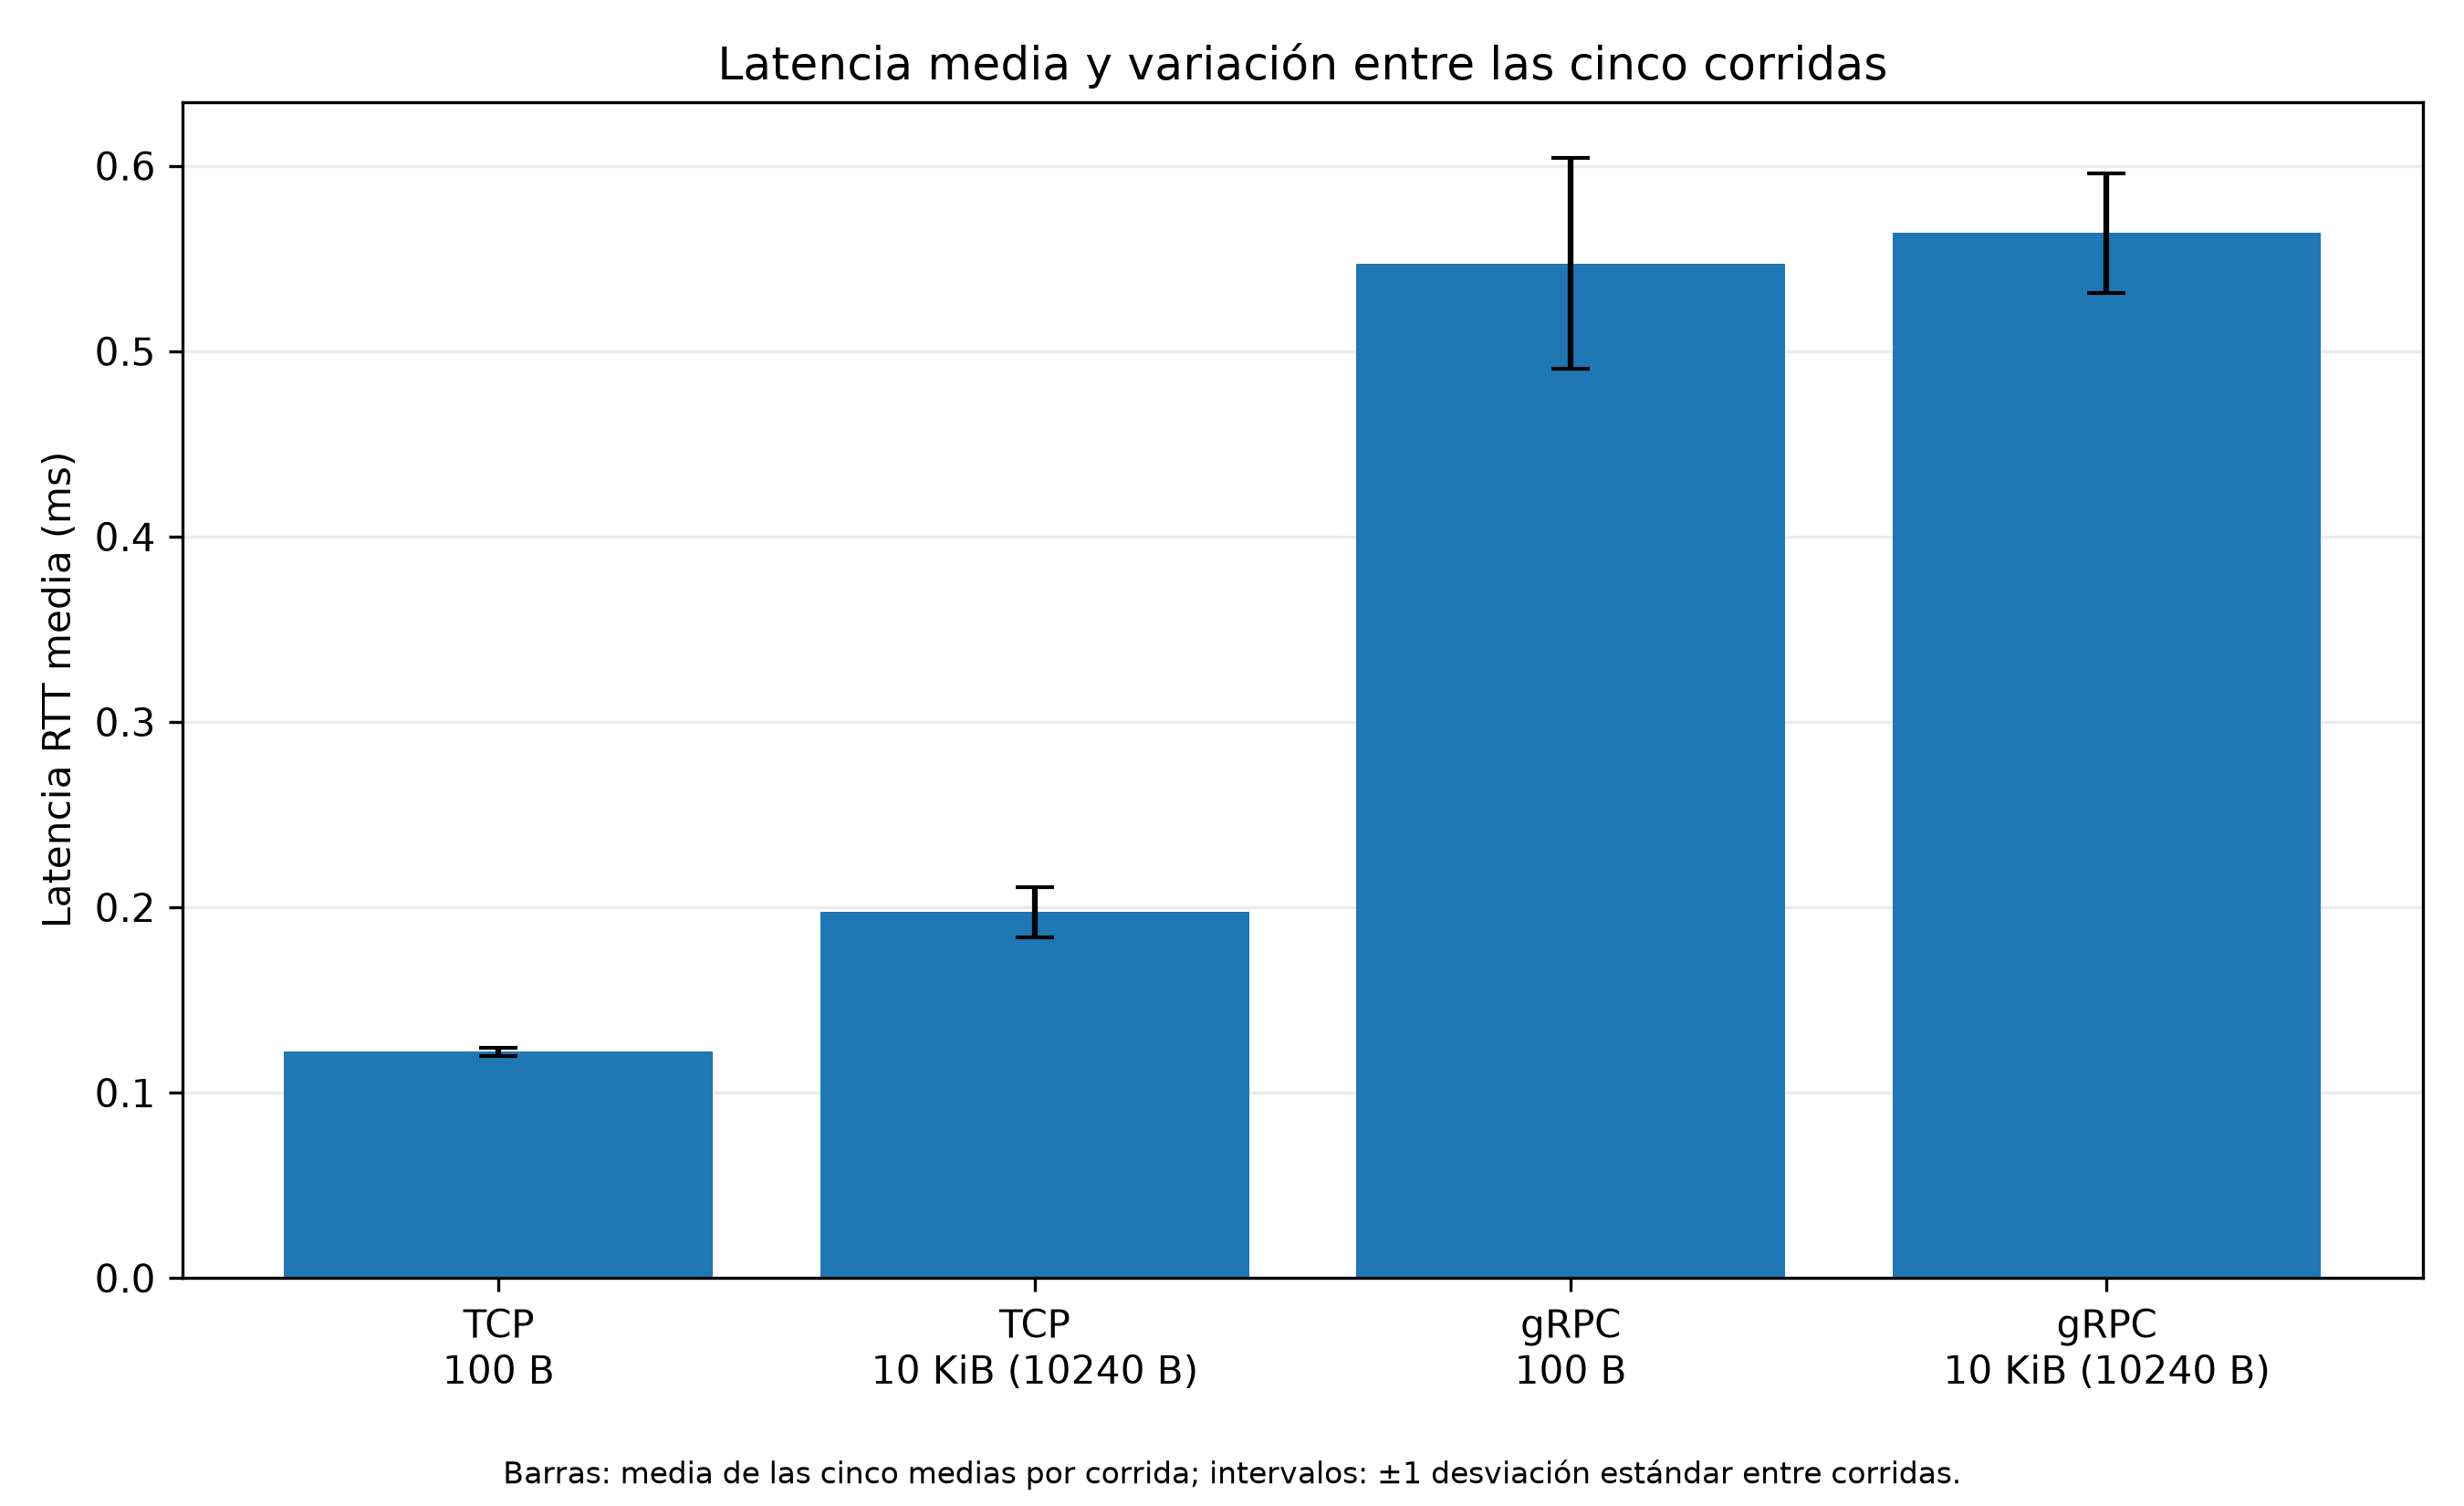
\includegraphics[width=0.85\linewidth]
    {figures/barras_intervalos.png}
    \caption{Comparación de las latencias medias.
    Los intervalos representan $\pm 1$ desviación
    estándar entre las cinco corridas y no son
    intervalos de confianza del 95\%.}
    \label{fig:barras}
\end{figure}

En el gráfico se puede observar que TCP mantuvo
una latencia media inferior a gRPC con los dos
tamaños de mensaje.

Las líneas de dispersión muestran que los tiempos
no fueron exactamente iguales en todas las
corridas. Esto se aprecia especialmente en gRPC
con mensajes de 100 bytes, donde hubo una mayor
diferencia entre las medias de las repeticiones.

Estos intervalos sirven para mostrar cuánto
variaron los resultados entre corridas.
No se utilizaron para realizar una prueba
de significación estadística.

\subsection{Alcance de los resultados y concurrencia}

Las veinte corridas del benchmark se completaron
correctamente. En los archivos consolidados
se registraron 2000 mediciones válidas,
sin acuses fallidos ni latencias inválidas.

Estos valores corresponden a mensajes enviados
de forma secuencial entre el cliente
\texttt{nodo-A} y el servidor \texttt{nodo-B}.
Por tanto, las cifras de latencia y rendimiento
presentadas anteriormente no describen por
sí solas el comportamiento con tres clientes
concurrentes.

En las pruebas funcionales posteriores se
registraron veinte intercambios por mecanismo,
con tres nodos en funcionamiento. Tanto TCP
como gRPC completaron las veinte solicitudes
y sus acuses. Cada ejecución produjo 80
eventos y 40 pares de envío y recepción,
sin errores causales en el informe de
verificación.

Para evaluar la concurrencia se realizaron
cuatro pruebas adicionales, con cargas de
100 y 10240 bytes para ambos mecanismos.
En cada condición se registraron 300
solicitudes, 300 acuses y 1200 eventos.
Los informes de verificación no reportaron
errores causales en estas capturas.

Estos resultados muestran que las
implementaciones completaron los intercambios
registrados bajo las condiciones probadas.
Aunque las pruebas con tres clientes se completaron
correctamente, no se utilizaron para comparar
latencias ni mensajes por segundo con el benchmark
inicial. Su objetivo fue comprobar la comunicación
entre los nodos y verificar los relojes de Lamport,
además de haberse ejecutado en un entorno diferente.

La verificación de las reglas de Lamport,
los ejemplos de eventos concurrentes y
la procedencia de los registros se
presentan con mayor detalle en la
sección de verificación del reloj lógico.

